\chapter{Marco Teórico}
	\label{sec:teorico}




\section{Teoría de Sistemas Dinámicos y Control}

El análisis y diseño de Sistemas Ciberfísicos (CPS) requiere una modelación matemática rigurosa de los procesos físicos involucrados. En esta sección se establecen las definiciones fundamentales de la teoría de sistemas orientada al control continuo, estructurando las nociones de variables dinámicas, clasificaciones de sistemas y sus representaciones matemáticas.

\subsection{Concepto de Sistema, Entradas, Estados y Salidas}

Desde la perspectiva de la teoría de control, un \textit{sistema} es una entidad abstracta o física que procesa señales de entrada para producir señales de salida a lo largo del tiempo. Matemáticamente, este comportamiento se describe mediante una representación en el \textbf{espacio de estados}, la cual modela la dinámica interna del proceso a través de un conjunto de variables de primer orden de la siguiente forma:

\begin{equation}
    \dot{x}(t) = f(x(t), u(t), w(t), t)
    \label{eq:estado_general}
\end{equation}
\begin{equation}
    y(t) = g(x(t), u(t), w(t), t)
    \label{eq:salida_general}
\end{equation}

Donde las variables e interacciones principales se definen formalmente como:
\begin{itemize}
    \item \textbf{Vector de Estados ($x(t) \in \mathbb{R}^{n_x}$):} Representa la memoria interna del sistema, con $n_x$ el orden o dimensión del sistema. Contiene el conjunto mínimo de variables independientes cuyo conocimiento en un instante inicial $t_0$, junto con las entradas aplicadas para $t \ge t_0$, determina unívocamente el comportamiento futuro del sistema.
    \item \textbf{Vector de Entradas de Control ($u(t) \in \mathbb{R}^{n_u}$):} Representa las señales de actuación que el diseñador o controlador puede manipular directamente para modificar la trayectoria de los estados del sistema, con $n_u$ el número de actuadores disponibles.
    \item \textbf{Vector de Perturbaciones ($w(t) \in \mathbb{R}^{n_w}$):} Representa señales exógenas no controlables que afectan la dinámica del proceso físico. Estas señales modelan ruidos ambientales, errores de modelado o fuerzas externas imprevistas.
    \item \textbf{Vector de Salidas ($y(t) \in \mathbb{R}^{n_y}$):} Representa las variables medibles o de interés operativo del sistema. Comúnmente corresponde a combinaciones de los estados que son capturadas por sensores.
\end{itemize}

Las Ecuaciones~\eqref{eq:estado_general}-\eqref{eq:salida_general} son completamente generales y admiten dinámicas no lineales arbitrarias a través de las funciones $f(\cdot)$ y $g(\cdot)$. La siguiente subsección presenta, a modo de preámbulo, el caso particular en que estas funciones son lineales y no dependen del tiempo; este caso clásico permite introducir con la menor complejidad posible las nociones de estabilidad y de función de Lyapunov que, más adelante, se generalizarán al caso de interés de esta memoria: los sistemas con parámetros variables en el tiempo.

\subsection{Preámbulo: Sistemas Lineales Invariantes en el Tiempo (LTI)}


Un sistema dinámico se clasifica como \textit{Lineal Invariante en el Tiempo} (LTI, por sus siglas en inglés) si satisface los principios de superposición (homogeneidad y aditividad) y sus parámetros internos no varían de manera explícita con respecto al tiempo. En el espacio de estados continuo, un sistema lineal acoplado con entradas de control y señales de perturbación adopta la siguiente estructura matricial compacta:

\begin{equation}
    \dot{x}(t) = A x(t) + B u(t) + B_w w(t)
    \label{eq:estado_lti}
\end{equation}
\begin{equation}
    y(t) = C x(t) + D u(t) + D_w w(t)
    \label{eq:salida_lti}
\end{equation}

Donde las componentes deterministas del sistema están representadas por matrices de dimensiones apropiadas:
\begin{itemize}
    \item $A \in \mathbb{R}^{n_x \times n_x}$ es la matriz del sistema o matriz de dinámica interna.
    \item $B \in \mathbb{R}^{n_x \times n_u}$ es la matriz de entrada de control.
    \item $B_w \in \mathbb{R}^{n_x \times n_w}$ es la matriz de perturbación exógena.
    \item $C \in \mathbb{R}^{n_y \times n_x}$ es la matriz de salida o de observación.
    \item $D \in \mathbb{R}^{n_y \times n_u}$ y $D_w \in \mathbb{R}^{n_y \times n_w}$ son las matrices de transmisión directa.
\end{itemize}

Un concepto central para los sistemas LTI es la \textit{estabilidad asintótica}. En ausencia de entradas ($u(t) = 0, w(t) = 0$), la dinámica autónoma del sistema queda definida exclusivamente por la ecuación diferencial lineal homogénea $\dot{x}(t) = A x(t)$. La solución analítica de este sistema, dada una condición inicial $x(0) = x_0$, viene determinada por la matriz exponencial:

\begin{equation}
    x(t) = e^{At} x_0
    \label{eq:sol_lti}
\end{equation}

Para comprender el comportamiento cualitativo de esta solución, se recurre al análisis espectral de la matriz del sistema $A \in \mathbb{R}^{n_x \times n_x}$. Los valores propios (o autovalores) $\lambda_i$ de $A$ son las raíces del polinomio característico definido por $\det(\lambda I - A) = 0$. En el caso general, estos valores propios pueden ser reales o complejos conjugados, adoptando la forma:

\begin{equation}
    \lambda_i = \sigma_i + j\omega_i
    \label{eq:autovalor_complejo}
\end{equation}

donde $\sigma_i = \text{Re}(\lambda_i)$ representa la parte real y $\omega_i = \text{Im}(\lambda_i)$ la parte imaginaria. Si la matriz $A$ es diagonalizable, existe una matriz de transformación de similitud $V$ compuesta por los vectores propios de $A$ tal que $A = V \Lambda V^{-1}$, donde $\Lambda = \text{diag}(\lambda_1, \lambda_2, \dots, \lambda_{n_x})$. Bajo este cambio de coordenadas, la respuesta temporal del sistema se puede descomponer como una combinación lineal de los modos dinámicos individuales:

\begin{equation}
    x(t) = \sum_{i=1}^{n_x} v_i c_i e^{\lambda_i t} = \sum_{i=1}^{n_x} v_i c_i e^{\sigma_i t} \left( \cos(\omega_i t) + j\sin(\omega_i t) \right)
    \label{eq:modos_dinamicos}
\end{equation}

donde $v_i$ representan los vectores propios y $c_i$ son constantes que dependen de las condiciones iniciales. A partir de esta descomposición, se puede observar que el comportamiento asintótico del sistema cuando $t \to \infty$ está gobernado estrictamente por el término exponencial real $e^{\sigma_i t}$. 

Por lo tanto, el sistema es de tipo \textit{Hurwitz} (o internamente estable de manera asintótica:) si y solo si todos los valores propios de la matriz de dinámica $A$ poseen partes reales estrictamente negativas, siendo esta la expresión:

\begin{equation}
    \text{Re}(\lambda_i(A)) < 0, \quad \forall i \in \{1, \dots, n_x\}
    \label{eq:condicion_hurwitz}
\end{equation}

Si esta condición se cumple, el término $e^{\sigma_i t}$ decae exponencialmente hacia cero, garantizando que $\lim_{t \to \infty} x(t) = 0$ ante cualquier condición inicial $x_0$. Por el contrario, si existe al menos un valor propio con $\text{Re}(\lambda_i) > 0$, el modo dinámico asociado crecerá de forma ilimitada, resultando en un sistema inestable. En el caso de que existan autovalores sobre el eje imaginario ($\text{Re}(\lambda_i) = 0$), el sistema presentará oscilaciones sostenidas o respuestas marginalmente estables. Esta relación geométrica entre la ubicación de los autovalores en el plano complejo y la naturaleza de las trayectorias del estado se ilustra en la Figura~\ref{fig:estabilidad_plano}.

\begin{figure}[ht]
    \centering
    % Asegúrate de descomentar \usepackage{tikz} en el preámbulo de tu documento
    \begin{subfigure}{\textwidth}
    \centering
    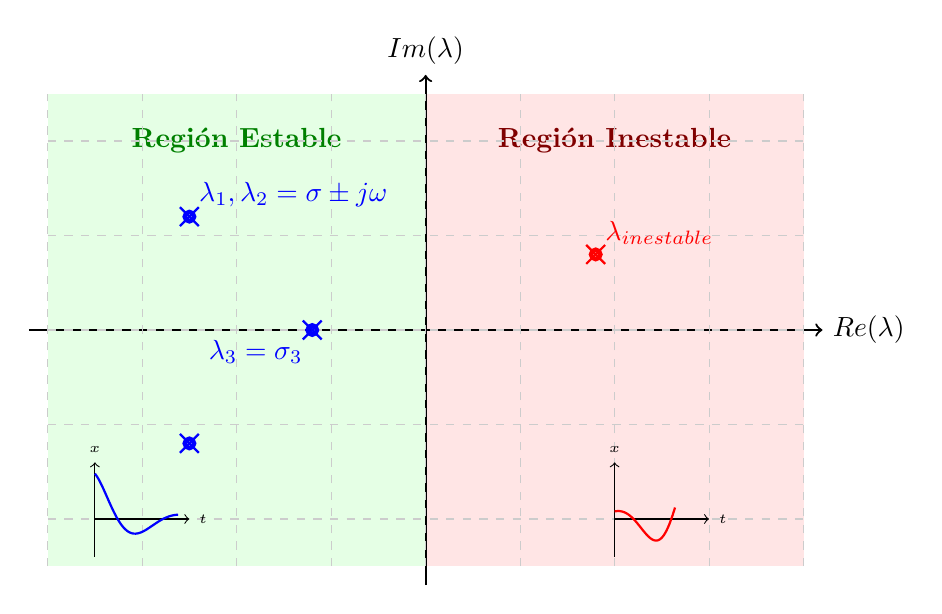
\begin{tikzpicture}[scale=1.2]
        % Fondo de la región de estabilidad (Semiplano izquierdo)
        \fill[green!10] (-4,-2.5) rectangle (0,2.5);
        \node[green!50!black] at (-2,2) {\textbf{Región Estable}};
        
        % Fondo de la región de inestabilidad (Semiplano derecho)
        \fill[red!10] (0,-2.5) rectangle (4,2.5);
        \node[red!50!black] at (2,2) {\textbf{Región Inestable}};

        % Ejes coordenados
        \draw[->,thick] (-4.2,0) -- (4.2,0) node[right] {$\text{Re}(\lambda)$};
        \draw[->,thick] (0,-2.7) -- (0,2.7) node[above] {$\text{Im}(\lambda)$};
        
        % Líneas de división de cuadrículas atenuadas
        \draw[dashed, gray!40] (-4,-2.5) grid (4,2.5);

        % Autovalores estables (Cruces en la izquierda)
        \draw[ultra thick, blue] (-2.5,1.2) circle (0.05);
        \draw[thick, blue] (-2.6,1.1) -- (-2.4,1.3);
        \draw[thick, blue] (-2.6,1.3) -- (-2.4,1.1);
        \node[blue, above right] at (-2.5,1.2) {$\lambda_1, \lambda_2 = \sigma \pm j\omega$};
        
        \draw[ultra thick, blue] (-2.5,-1.2) circle (0.05);
        \draw[thick, blue] (-2.6,-1.3) -- (-2.4,-1.1);
        \draw[thick, blue] (-2.6,-1.1) -- (-2.4,-1.3);

        \draw[ultra thick, blue] (-1.2,0) circle (0.05);
        \draw[thick, blue] (-1.3,-0.1) -- (-1.1,0.1);
        \draw[thick, blue] (-1.3,0.1) -- (-1.1,-0.1);
        \node[blue, below left] at (-1.2,0) {$\lambda_3 = \sigma_3$};

        % Autovalor inestable (Cruz en la derecha)
        \draw[ultra thick, red] (1.8,0.8) circle (0.05);
        \draw[thick, red] (1.7,0.7) -- (1.9,0.9);
        \draw[thick, red] (1.7,0.9) -- (1.9,0.7);
        \node[red, above right] at (1.8,0.8) {$\lambda_{inestable}$};

        % Pequeños gráficos de comportamiento temporal embebidos
        % Mini gráfico estable
        \begin{scope}[shift={(-3.5,-2)}, scale=0.4]
            \draw[->] (0,0) -- (2.5,0) node[right] {\tiny $t$};
            \draw[->] (0,-1) -- (0,1.5) node[above] {\tiny $x$};
            \draw[thick, blue, domain=0:2.2, samples=50] plot (\x, {1.2*exp(-\x)*cos(150*\x)});
        \end{scope}
        
        % Mini gráfico inestable
        \begin{scope}[shift={(2,-2)}, scale=0.4]
            \draw[->] (0,0) -- (2.5,0) node[right] {\tiny $t$};
            \draw[->] (0,-1) -- (0,1.5) node[above] {\tiny $x$};
            \draw[thick, red, domain=0:1.6, samples=50] plot (\x, {0.2*exp(\x)*cos(180*\x)});
        \end{scope}
    \end{tikzpicture}
    \end{subfigure}
    \caption{Representación espectral de la estabilidad en el plano complejo $\mathbb{C}$. El semiplano izquierdo representa el espacio geométrico donde los autovalores de una matriz de Hurwitz inducen trayectorias dinámicas asintóticamente convergentes a cero.}
    \label{fig:estabilidad_plano}
\end{figure}

Este preámbulo LTI establece dos herramientas conceptuales que reutilizaremos a lo largo de todo el marco teórico: (i) la estabilidad se certifica mediante el signo de los autovalores de la matriz de dinámica, y (ii) esta condición espectral admite una formulación algebraica equivalente en términos de una matriz definida positiva $P$, que desarrollaremos formalmente en la Sección~\ref{sec:lyapunov_lmi}. A partir de este punto, el marco teórico abandona la matriz constante $A$ propia del caso LTI y trabaja exclusivamente con la estructura de parámetros variables que sí corresponde al sistema de interés de este estudio.

\section{Sistemas Lineales de Parámetros Variables (LPV) y Modelos Parametrizados}
\label{sec:lpv}

Los procesos reales en los CPS a menudo operan bajo condiciones cambiantes, variaciones estructurales o dependencias operativas no lineales. Para capturar este comportamiento sin perder las ventajas de las herramientas lineales, se recurre a la formulación de \textit{Sistemas Lineales de Parámetros Variables} (LPV) o sistemas parametrizados.

En este marco de modelación, la dinámica del sistema depende explícitamente de un vector de parámetros externos o variables de operación variables en el tiempo, denotado por $\xi(t) \in \mathbb{R}^p$. La representación en espacio de estados de la Ecuación~\eqref{eq:estado_general} se particulariza entonces a la forma \textit{lineal de parámetros variables}, en la cual las funciones $f(\cdot)$ y $g(\cdot)$ dejan de ser arbitrarias y adoptan una estructura afín en $(x(t), u(t), w(t))$, pero cuyos coeficientes —las matrices del sistema— ya no son constantes, sino que se transforman en funciones del parámetro operativo $\xi(t)$:

\begin{equation}
    \dot{x}(t) = f(x(t), u(t), w(t), \xi(t)) = A(\xi(t)) x(t) + B(\xi(t)) u(t) + B_w(\xi(t)) w(t)
    \label{eq:estado_lpv}
\end{equation}
\begin{equation}
    y(t) = g(x(t), u(t), w(t), \xi(t)) = C(\xi(t)) x(t) + D(\xi(t)) u(t) + D_w(\xi(t)) w(t)
    \label{eq:salida_lpv}
\end{equation}

Las Ecuaciones~\eqref{eq:estado_lpv}-\eqref{eq:salida_lpv} constituyen la representación general del sistema LPV que se utilizará a lo largo del estudio.

El vector de parámetros $\xi(t)$ suele variar dentro de un conjunto compacto admisible $\Xi \subset \mathbb{R}^p$. Esta formulación permite modelar situaciones críticas en CPS como:
\begin{enumerate}
    \item \textbf{Variaciones estructurales:} Cambios físicos intrínsecos en el sistema, tales como variaciones de masa, fluctuaciones térmicas o cambios en la resistencia de componentes debidos al desgaste.
    \item \textbf{Linealización alrededor de trayectorias (Ganancia Programada):} Aproximaciones locales de sistemas altamente no lineales a lo largo de diferentes puntos de operación indexados por la variable $\xi$.
    \item \textbf{Ciberataques y anomalías en la red:} En el contexto de los CPS, ataques maliciosos como la inyección de datos falsos (FDI), ataques de denegación de servicio (DoS) o el secuestro de actuadores pueden alterar la topología de comunicación o modificar los parámetros efectivos del sistema físico, lo cual se modela mediante cambios abruptos y arbitrarios en el vector $\xi(t)$ \cite{pasqualetti2013attack, cardenas2008secure}.
\end{enumerate}

El principal desafío operativo bajo el enfoque LPV es que las condiciones de estabilidad deben garantizarse de forma unívoca para \textit{cualquier} trayectoria posible que el parámetro $\xi(t)$ adopte dentro del espacio admisible $\Xi$. En este contexto, una \textbf{trayectoria paramétrica} se define como una función dependiente del tiempo $\xi: [0, \infty) \to \Xi$, la cual describe el historial de la evolución del punto de operación o el perfil temporal de una anomalía. Garantizar la estabilidad robusta implica asegurar que el estado del sistema converja o permanezca acotado sin importar qué camino específico tome $\xi(t)$, ni cuán rápido varíe dentro de los límites de $\Xi$. La trayectoria paramétrica $\xi(t)$ se ilustra en la Figura~\ref{fig:politopo_limites}, donde se muestra su recorrido dentro del espacio admisible.

A diferencia de los sistemas LTI, donde la estabilidad se certifica evaluando el espectro fijo de la matriz $A$, los sistemas LPV presentan un desafío mayor. Un teorema fundamental en sistemas variables en el tiempo establece que el hecho de que los autovalores de $A(\xi)$ posean partes reales negativas para cada parámetro ``congelado'' en $\Xi$, \textbf{no garantiza} la estabilidad del sistema dinámico; fluctuaciones paramétricas suficientemente rápidas pueden inducir inestabilidad.

Por lo tanto, para el caso de un sistema LPV se exige generalizar una función de Lyapunov. Se dice que un sistema es \textit{cuadráticamente estabilizable} si admite una función de Lyapunov cuadrática común $V(x) = x^T P x$ que disipe energía bajo cualquier condición. Hallarla implica encontrar una única matriz $P \in \mathbb{S}^n$ que satisfaga la restricción para todo el dominio de operación simultáneamente:

\begin{equation}
    P \succ 0
    \label{eq:P_positiva_lpv}
\end{equation}
\begin{equation}
    A(\xi)^T P + P A(\xi) \prec 0, \quad \forall \xi \in \Xi
    \label{eq:lyap_lpv_infinita}
\end{equation}

Dado que el conjunto $\Xi$ es continuo y contiene infinitos puntos, la Ecuación~\eqref{eq:lyap_lpv_infinita} representa un problema de optimización semidefinida de dimensión infinita, lo cual es computacionalmente intratable de resolver directamente. 

\subsection{Estabilidad de Sistemas LPV mediante Modelos Politópicos}

Para sortear este obstáculo de dimensionalidad infinita, una de las maneras que propone la literatura de control robusto para lograr la estabilidad en sistemas LPV es la representación mediante polítopos \rev{\cite{boyd1994lmi, apkarian2000parameterized}}. Geométricamente, un polítopo es la generalización de un polígono (en 2D) o un poliedro (en 3D) a $p$ dimensiones. En el modelado de sistemas, el polítopo define los límites máximos y mínimos que pueden tomar los parámetros físicos. 

Los \textbf{vértices del polítopo} ($N$) corresponden a las combinaciones de las condiciones operativas extremas (o ``peores casos''). Por ejemplo, si un sistema depende de una masa $m \in [m_{min}, m_{max}]$ y una fricción $f \in [f_{min}, f_{max}]$, el espacio admisible $\Xi$ es un rectángulo cuyos $N=4$ vértices son las combinaciones de dichos valores extremos. 

\begin{figure}[ht]
    \centering
    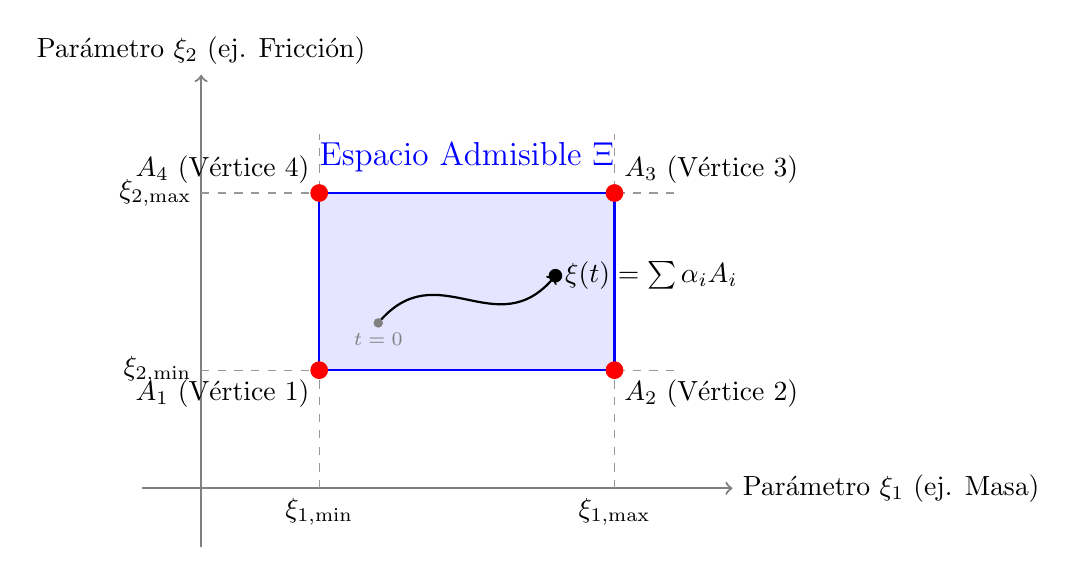
\begin{tikzpicture}[scale=1.5]
        % Ejes de los parámetros
        \draw[->, thick, gray] (-0.5, 0) -- (4.5, 0) node[right, text=black] {Parámetro $\xi_1$ (ej. Masa)};
        \draw[->, thick, gray] (0, -0.5) -- (0, 3.5) node[above, text=black] {Parámetro $\xi_2$ (ej. Fricción)};

        % Líneas de los límites operativos (mínimos y máximos)
        \draw[dashed, gray!80] (1,0) node[below, text=black] {$\xi_{1,\min}$} -- (1,3);
        \draw[dashed, gray!80] (3.5,0) node[below, text=black] {$\xi_{1,\max}$} -- (3.5,3);
        \draw[dashed, gray!80] (0,1) node[left, text=black] {$\xi_{2,\min}$} -- (4,1);
        \draw[dashed, gray!80] (0,2.5) node[left, text=black] {$\xi_{2,\max}$} -- (4,2.5);

        % Área del polítopo (Región de operación admisible Xi)
        \filldraw[fill=blue!10, draw=blue, thick] (1,1) rectangle (3.5,2.5);

        % Vértices (Los modelos en los peores casos / extremos)
        \filldraw[red] (1,1) circle (2pt) node[below left, text=black] {$A_1$ (Vértice 1)};
        \filldraw[red] (3.5,1) circle (2pt) node[below right, text=black] {$A_2$ (Vértice 2)};
        \filldraw[red] (3.5,2.5) circle (2pt) node[above right, text=black] {$A_3$ (Vértice 3)};
        \filldraw[red] (1,2.5) circle (2pt) node[above left, text=black] {$A_4$ (Vértice 4)};

        % Trayectoria del parámetro en el interior
        \draw[thick, black, ->] (1.5, 1.4) .. controls (2, 2) and (2.5, 1.2) .. (3, 1.8);
        \filldraw[black] (3, 1.8) circle (1.5pt) node[right] {$\xi(t) = \sum \alpha_i A_i$};
        \filldraw[gray] (1.5, 1.4) circle (1pt) node[below] {\scriptsize $t=0$};

        % Etiqueta del conjunto
        \node[blue, font=\large] at (2.25, 2.8) {Espacio Admisible $\Xi$};
    \end{tikzpicture}
    \caption{Representación geométrica de un polítopo paramétrico en 2D. Las líneas punteadas representan los límites físicos o restricciones operativas del sistema. La intersección de estos límites define los vértices ($A_i$), correspondientes a las condiciones operativas extremas. Cualquier variación en el tiempo del sistema físico ($\xi(t)$) queda contenida de forma segura dentro de la región azul, expresable como combinación convexa de sus vértices.}
    \label{fig:politopo_limites}
\end{figure}

Si se asume que la matriz del sistema $A(\xi)$ depende de forma afín de los parámetros $\xi$, entonces cualquier matriz del sistema evaluada en un punto de operación intermedio puede expresarse como una \textit{combinación convexa} de las matrices evaluadas en los vértices extremos, denotadas como $A_i$:

\begin{equation}
    A(\xi) = \sum_{i=1}^{N} \alpha_i A_i, \quad \text{con } \sum_{i=1}^{N} \alpha_i = 1, \quad \alpha_i \ge 0
    \label{eq:combinacion_convexa}
\end{equation}

Bajo esta transformación, y gracias a la linealidad geométrica de las LMIs, se demuestra que si una desigualdad matricial estricta se cumple en todos los vértices de un polítopo, automáticamente se cumple para cualquier punto en su interior. Así, el problema de infinitas restricciones de la Ecuación~\eqref{eq:lyap_lpv_infinita} se reduce de forma exacta a un conjunto finito de $N$ LMIs acopladas:

\begin{equation}
    A_i^T P + P A_i \prec 0, \quad \forall i \in \{1, 2, \dots, N\}
    \label{eq:lmi_politopica_finita}
\end{equation}

Encontrar una matriz $P$ que resuelva este conjunto finito de LMIs garantiza que el sistema LPV se mantenga asintóticamente estable para toda posible variación temporal de $\xi(t)$. Sin embargo, a medida que la dimensión del sistema ($n_x$) o la cantidad de parámetros inciertos crecen, el número de vértices $N$ aumenta exponencialmente. El costo computacional de resolver este conjunto acoplado de restricciones mediante solucionadores de punto interior en tiempo real se vuelve prohibitivo para las dinámicas rápidas de los CPS.








\section{Desigualdades Matriciales Lineales y Teoría de Lyapunov}
\label{sec:lyapunov_lmi}

Introduciremos desde sus bases el concepto de Desigualdad Matricial Lineal (LMI) y el Método Directo de Lyapunov, cuya intersección constituye la base del control robusto moderno. Para desarrollar estas herramientas con la menor carga notacional posible, esta sección introduce primero los conceptos de positividad matricial y de función de Lyapunov sobre la matriz constante $A$ del caso LTI; la generalización de estos resultados a la matriz dependiente de parámetros $A(\xi)$ y a su versión politópica $A_i$ se retoma en la Sección~\ref{sec:lazo_cerrado}, donde se formula el problema de síntesis de control propiamente LPV.

\subsection{Fundamentos de las Desigualdades Matriciales Lineales (LMI)}

En el ámbito del álgebra lineal y la optimización, una Desigualdad Matricial Lineal (LMI, por sus siglas en inglés) es una condición que restringe el espacio de soluciones de un problema. Su propósito es garantizar que una matriz paramétrica, cuyos elementos dependen de un conjunto de variables desconocidas (variables de decisión), resulte ser definida positiva (o negativa). 

Se dice que la matriz está construida \textbf{paramétricamente} porque no está compuesta por valores numéricos estáticos, sino que se formula como una función afín de ciertos parámetros de diseño. En el contexto de la teoría de control, esta parametrización es fundamental: los parámetros desconocidos representan precisamente las incógnitas que un ingeniero o un algoritmo deben encontrar (por ejemplo, los coeficientes de un controlador o los elementos de una función de Lyapunov). Al estructurar estas incógnitas de forma lineal dentro de la matriz, el problema de buscar un diseño estable se transforma en un problema de búsqueda geométrica. La principal ventaja de formular el problema de esta manera es que el conjunto de parámetros que satisface la LMI forma un espacio de soluciones estrictamente convexo, lo que garantiza la tratabilidad computacional y la inexistencia de mínimos locales al optimizar.

\subsection*{Positividad}
Sea $P \in \mathbb{S}^n$ una matriz cuadrada y simétrica (es decir, $P = P^T$). Se dice que $P$ es \textbf{definida positiva}, denotado como $P \succ 0$, si para cualquier vector no nulo $x \in \mathbb{R}^n$, la forma cuadrática asociada es estrictamente mayor que cero:

\begin{equation}
    x^T P x > 0, \quad \forall x \neq 0
    \label{eq:def_positiva}
\end{equation}

Para comprender el impacto geométrico de la matriz $P$, es imperativo analizar su estructura a través del teorema espectral. Toda matriz simétrica $P \in \mathbb{S}^n$ puede descomponerse en la forma $P = V \Lambda V^T$, donde $\Lambda$ es una matriz diagonal que contiene los valores propios (o autovalores) $\lambda_i$, y $V$ es una matriz ortogonal cuyas columnas son los vectores propios (o autovectores) de $P$.

En el contexto de la función de energía $V(x) = x^T P x = c$, estos elementos dictan completamente la topología del espacio de estados:
\begin{itemize}
    \item \textbf{Los vectores propios ortogonales ($v_i$):} Representan los ejes principales o ``direcciones naturales'' de la figura geométrica. Al ser ortogonales (forman ángulos de $90^\circ$ entre sí en el espacio de dimensión $n$), garantizan que la matriz define un sistema de coordenadas no distorsionado. Físicamente, indican las direcciones en las que la dinámica del sistema está puramente desacoplada.
    \item \textbf{Los valores propios ($\lambda_i$):} Representan el factor de concavidad o ``escala'' a lo largo de cada vector propio. La longitud del semieje de la figura geométrica en la dirección del vector propio $v_i$ está dada por $\frac{\sqrt{c}}{\sqrt{\lambda_i}}$. 
\end{itemize}

Si la matriz $P$ es definida positiva, todos sus valores propios son estrictamente mayores que cero ($\lambda_i > 0$). Esto asegura que todas las longitudes de los semiejes sean números reales finitos. En consecuencia, la ecuación $x^T P x = c$ forma un elipsoide cerrado centrado en el origen. Desde la perspectiva del control, esto significa que la ``energía'' del sistema está confinada, lo que se traduce en que el estado $x(t)$ no puede escapar hacia el infinito sin aumentar el nivel de energía $c$ como se aprecia en la figura~\ref{fig:elipsoide_P_pos}.

Por el contrario, si $P$ pierde su positividad y presenta al menos un autovalor negativo, la longitud de ese semieje se vuelve imaginaria. Geométricamente, el elipsoide se ``rompe'' y se abre transformándose en un hiperboloide (ver figura~\ref{fig:elipsoide_P_indef}). Físicamente, esto es catastrófico para la estabilidad: implica que el sistema posee trayectorias a lo largo de las cuales los estados pueden crecer de forma ilimitada (hacia el infinito) mientras la ``energía'' medida $c$ se mantiene constante o incluso disminuye, violando el principio de confinamiento de Lyapunov.

\begin{figure}[ht]
    \centering
    % ---------- SUBFIGURA 1: MATRIZ DEFINIDA POSITIVA (Elipse) ----------
    \begin{subfigure}{0.48\textwidth}
        \centering
        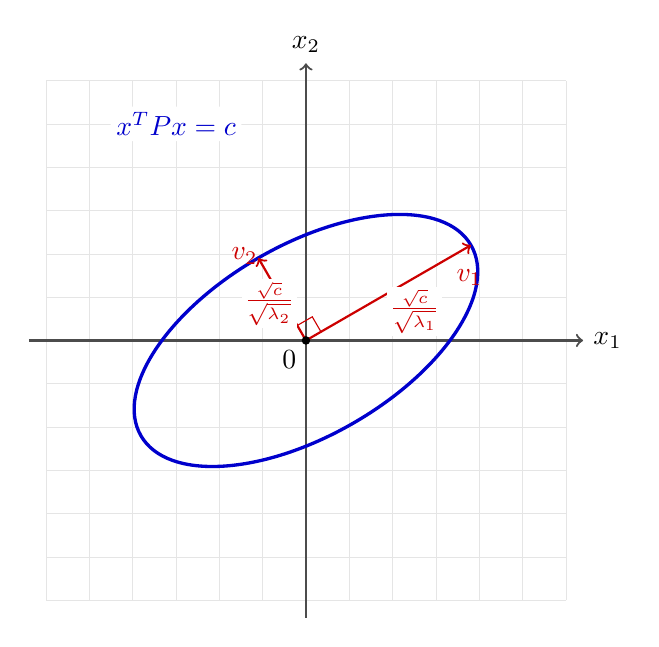
\begin{tikzpicture}[scale=1.1]
            % Cuadrícula de fondo suave
            \draw[step=0.5cm, gray!20, very thin] (-3,-3) grid (3,3);
            
            % Ejes de coordenadas
            \draw[->, thick, black!70] (-3.2, 0) -- (3.2, 0) node[right, text=black] {$x_1$};
            \draw[->, thick, black!70] (0, -3.2) -- (0, 3.2) node[above, text=black] {$x_2$};
            
            % Elipse (Rotada 30 grados)
            \draw[very thick, blue!80!black, rotate=30] (0,0) ellipse (2.2cm and 1.1cm);
            
            % Vectores Propios (Ejes ortogonales)
            \draw[->, thick, red!80!black] (0,0) -- (30:2.2) node[pos=0.85, below right] {$v_1$};
            \draw[->, thick, red!80!black] (0,0) -- (120:1.1) node[pos=0.8, above left] {$v_2$};
            
            % Etiquetas de longitudes
            \node[red!80!black, fill=white, inner sep=1pt] at (15:1.3) {\footnotesize $\frac{\sqrt{c}}{\sqrt{\lambda_1}}$};
            \node[red!80!black, fill=white, inner sep=1pt] at (135:0.6) {\footnotesize $\frac{\sqrt{c}}{\sqrt{\lambda_2}}$};
            
            % Origen y ángulo recto
            \filldraw[black] (0,0) circle (1.2pt) node[below left] {$0$};
            \draw[red!80!black, thin, rotate=30] (0.2,0) -- (0.2,0.2) -- (0,0.2);
            
            % Ecuación
            \node[blue!80!black, fill=white, inner sep=2pt, rounded corners] at (-1.5, 2.5) {$x^T P x = c$};
        \end{tikzpicture}
        \caption{$P \succ 0$ (Autovalores $\lambda_1, \lambda_2 > 0$): La energía forma un elipsoide cerrado, confinando los estados.}
        \label{fig:elipsoide_P_pos}
    \end{subfigure}
    \hfill
    % ---------- SUBFIGURA 2: MATRIZ INDEFINIDA (Hipérbola) ----------
    \begin{subfigure}{0.48\textwidth}
        \centering
        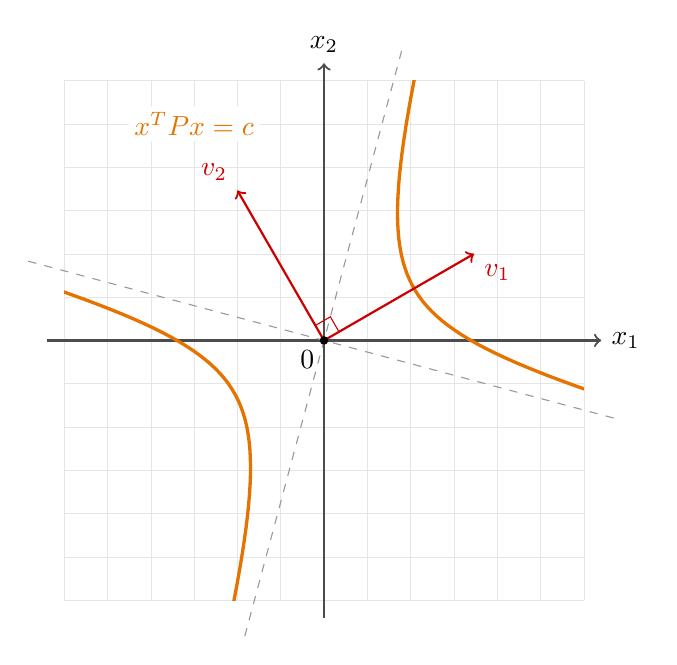
\begin{tikzpicture}[scale=1.1]
            % Cuadrícula de fondo suave
            \draw[step=0.5cm, gray!20, very thin] (-3,-3) grid (3,3);
            
            % Ejes de coordenadas
            \draw[->, thick, black!70] (-3.2, 0) -- (3.2, 0) node[right, text=black] {$x_1$};
            \draw[->, thick, black!70] (0, -3.2) -- (0, 3.2) node[above, text=black] {$x_2$};
            
            % Asíntotas de la hipérbola
            \draw[dashed, gray!80, rotate=30] (-2.5,-2.5) -- (2.5,2.5);
            \draw[dashed, gray!80, rotate=30] (-2.5,2.5) -- (2.5,-2.5);
            
            % Hipérbola (Dominio rotado 30 grados) - Representa lambda_1 > 0, lambda_2 < 0
            \clip (-3,-3) rectangle (3,3);
            \draw[very thick, orange!90!black, rotate=30, domain=-1.5:1.5, samples=50] plot ({1.2*cosh(\x)}, {1.2*sinh(\x)});
            \draw[very thick, orange!90!black, rotate=30, domain=-1.5:1.5, samples=50] plot ({-1.2*cosh(\x)}, {1.2*sinh(\x)});
            
            % Vectores Propios
            \draw[->, thick, red!80!black] (0,0) -- (30:2) node[below right] {$v_1$};
            \draw[->, thick, red!80!black] (0,0) -- (120:2) node[above left] {$v_2$};
            
            % Origen y ángulo recto
            \filldraw[black] (0,0) circle (1.2pt) node[below left] {$0$};
            \draw[red!80!black, thin, rotate=30] (0.2,0) -- (0.2,0.2) -- (0,0.2);
            
            % Ecuación
            \node[orange!90!black, fill=white, inner sep=2pt, rounded corners] at (-1.5, 2.5) {$x^T P x = c$};
        \end{tikzpicture}
        \caption{$P \not\succ 0$ (Ej: $\lambda_1 > 0, \lambda_2 < 0$): La superficie se abre en un hiperboloide. Existen trayectorias no acotadas.}
        \label{fig:elipsoide_P_indef}
    \end{subfigure}
    
    \caption{Interpretación geométrica de la matriz de Lyapunov $P$ mediante sus vectores propios ($v_1, v_2$) y la influencia de los signos de sus autovalores en el confinamiento del espacio de estados $\mathbb{R}^2$.}
    \label{fig:elipsoide_P}
\end{figure}

\subsection*{Linear Matrix Inequality (LMI)}

Una LMI general se formula estableciendo que una matriz afín, que depende de un vector de variables de decisión $y \in \mathbb{R}^m$, debe ser semidefinida o definida positiva. Su forma canónica es:

\begin{equation}
    F(y) = F_0 + y_1 F_1 + y_2 F_2 + \dots + y_m F_m \succ 0
    \label{eq:lmi_canonica}
\end{equation}

donde $F_0, F_1, \dots, F_m \in \mathbb{S}^n$ son matrices simétricas conocidas y $y_i$ son las incógnitas del problema. La propiedad más valiosa de una LMI es la convexidad: el conjunto de soluciones $y$ que satisfacen $F(y) \succ 0$ forma un conjunto estrictamente convexo. Esto implica que cualquier problema de optimización sujeto a restricciones LMI posee un único óptimo global, el cual puede ser hallado mediante algoritmos de punto interior.

\subsection{El Método Directo de Lyapunov}

A finales del siglo XIX, el matemático ruso Aleksandr Lyapunov formuló un método para determinar la estabilidad de un sistema dinámico sin necesidad de resolver analíticamente sus ecuaciones diferenciales. Este enfoque, conocido como el \textit{Método Directo de Lyapunov}, se basa en un principio físico fundamental: si la energía total de un sistema mecánico o eléctrico disipa (disminuye) continuamente a lo largo del tiempo, el sistema eventualmente se detendrá y alcanzará un punto de equilibrio estable.

Lyapunov propuso reemplazar el concepto físico de ``energía'' por una función matemática escalar abstracta $V(x)$, denominada \textit{función candidata de Lyapunov}, que depende del estado del sistema $x(t)$. Para que $V(x)$ sea válida, debe cumplir dos condiciones elementales:

\begin{enumerate}
    \item \textbf{Debe ser localmente definida positiva:} $V(x) > 0$ para todo $x \neq 0$, y $V(0) = 0$. Esto imita a la energía de un sistema, la cual es nula en el reposo y positiva en cualquier otro estado.
    \item \textbf{Su derivada temporal debe ser definida negativa:} A lo largo de las trayectorias del sistema, la variación de esta ``energía'' debe ser decreciente, es decir, $\dot{V}(x) < 0$ para todo $x \neq 0$.
\end{enumerate}

Si se logra encontrar al menos una función $V(x)$ que cumpla simultáneamente ambas condiciones para un sistema dado, el Teorema de Lyapunov garantiza matemática y rigurosamente que el origen del sistema es asintóticamente estable.

\subsection{De Lyapunov a LMI}

El nexo fundamental entre las abstracciones de Lyapunov, el álgebra matricial de las LMIs y, posteriormente, la teoría de control, surge al elegir una estructura matemática específica para la función de energía. La elección más clásica para la función candidata de Lyapunov es la forma cuadrática:

\begin{equation}
    V(x) = x^T P x
    \label{eq:lyap_cuadratica}
\end{equation}

Para satisfacer la primera condición de Lyapunov, basta con exigir directamente que la matriz $P$ sea definida positiva, lo que constituye nuestra primera desigualdad matricial. Ahora, supongamos un sistema dinámico lineal y autónomo descrito por la ecuación diferencial $\dot{x} = A x$. Para evaluar la segunda condición de Lyapunov, se debe derivar $V(x)$ con respecto al tiempo aplicando la regla de la cadena:

\begin{equation}
    \dot{V}(x) = \dot{x}^T P x + x^T P \dot{x}
    \label{eq:vdot_regla_cadena}
\end{equation}

Sustituyendo la dinámica del sistema ($\dot{x} = A x$) en la derivada, se obtiene:

\begin{equation}
    \dot{V}(x) = (A x)^T P x + x^T P (A x) = x^T A^T P x + x^T P A x
    \label{eq:vdot_sustitucion}
\end{equation}
\begin{equation}
    \dot{V}(x) = x^T \left( A^T P + P A \right) x
    \label{eq:vdot_cuadratica}
\end{equation}

Para que la energía disipe, se requiere que $\dot{V}(x) < 0$ para cualquier estado $x \neq 0$. Observando la Ecuación~\eqref{eq:vdot_cuadratica}, es evidente que esta condición se cumple si y solo si la matriz encerrada entre los vectores de estado es definida negativa. Esto genera nuestra segunda desigualdad matricial:

\begin{equation}
    A^T P + P A \prec 0
    \label{eq:lyap_lti}
\end{equation}

De esta manera, el problema abstracto y complejo de analizar ecuaciones diferenciales para demostrar la estabilidad de un sistema físico, ha sido transformado en un problema puramente algebraico. Si existe una matriz $P$ que satisfaga simultáneamente las LMIs $P \succ 0$ y $A^T P + P A \prec 0$, el sistema es estable. Esta traducción de dinámicas temporales a restricciones geométricas convexas es la base sobre la cual se diseñan los controladores robustos en la ingeniería de Sistemas Ciberfísicos.

La Ecuación~\eqref{eq:lyap_lti} corresponde al caso LTI, con la matriz constante $A$; su generalización directa al caso politópico corresponde a la Ecuación~\eqref{eq:lmi_politopica_finita}, reemplazando $A$ por cada vértice $A_i$ del polítopo y exigiendo una matriz $P$ común para todos ellos. De aquí en adelante, todas las LMIs se formulan directamente sobre la estructura politópica $A_i$, $B_i$ ($i=1,\dots,N$), pues es esta la que corresponde al sistema LPV objeto de este estudio.


















\section{Realimentación}
\label{sec:lazo_cerrado}


\subsection{El Principio de Realimentación y el Lazo Cerrado}

En la teoría de sistemas, una topología de control puede clasificarse fundamentalmente en dos paradigmas: lazo abierto (\textit{open-loop}) y lazo cerrado (\textit{closed-loop}). 

En una configuración de lazo abierto, la señal de control $u(t)$ inyectada al sistema físico (la planta) se calcula exclusivamente en función de una referencia deseada y un modelo matemático previo, sin tomar en cuenta el estado actual del sistema. Si bien es computacionalmente económica, esta arquitectura tiene la falencia de que si el modelo matemático posee imprecisiones o si perturbaciones externas las cuales normalmente se pueden presentar en la realidad como fricción no modelada, ráfagas de viento, sobrecalentamiento natural del sistema, etc, actúan sobre la planta, el error entre el estado real y el deseado crecerá sin que el controlador pueda detectarlo ni compensarlo.

Para dotar a los CPS de inteligencia y robustez, se emplea la arquitectura de lazo cerrado. En este esquema, el sistema de control mide continuamente a través de sensores el estado actual de la planta o sus salidas, y utiliza esta información para ajustar dinámicamente la señal de control $u(t)$. Este flujo continuo de información desde la salida hacia la entrada del controlador se denomina realimentación. La realimentación permite que el sistema se auto-corrija, compare su estado actual con un punto de equilibrio deseado, y genere la energía necesaria para anular cualquier desviación, mitigando eficazmente los efectos de las incertidumbres y perturbaciones exógenas. La Figura~\ref{fig:realimentacion} ilustra el esquema de realimentación de estados.

\begin{figure}[ht]
    \centering
    \begin{tikzpicture}[
        node distance=1.6cm,
        block/.style={draw, thick, rectangle, minimum height=1cm, minimum width=1.6cm, align=center},
        sum/.style={draw, thick, circle, minimum size=0.7cm, inner sep=0pt},
        >=latex
    ]
        % Nodos principales
        \node[sum] (sum) {};
        \node[block, right=of sum] (planta) {Planta\\ $\dot{x}=A(\xi)x+B(\xi)u$};
        \node[block, below=1.2cm of planta] (k) {$K$};
        \node[left=1.4cm of sum] (ref) {$r=0$};

        % Conexiones
        \draw[->, thick] (ref) -- node[above, pos=0.4] {} (sum);
        \draw[->, thick] (sum) -- node[above] {$u(t)$} (planta);
        \draw[->, thick] (planta) -- node[above] {$x(t)$} ++(2.4,0) coordinate (out);
        % Realimentación
        \draw[->, thick] (out) ++(-0.9,0) |- (k);
        \draw[->, thick] (k) -| (sum);
        % Signo del sumador
        \node at ($(sum)+(-0.18,0.18)$) {\scriptsize $+$};
        \node at ($(sum)+(-0.18,-0.2)$) {\scriptsize $+$};
    \end{tikzpicture}
    \caption{Esquema de realimentación de estados aplicado al sistema politópico. El controlador estático $K$ mide el vector de estado $x(t)$ y genera la señal de control $u(t)=Kx(t)$, que se reinyecta a la planta para conformar la dinámica en lazo cerrado $\dot{x}=(A(\xi)+B(\xi)K)x$. Nótese que la misma ganancia $K$ debe estabilizar la planta para toda variación admisible de $\xi(t)$.}
    \label{fig:realimentacion}
\end{figure}

\subsection{Realimentación de Estados y Asignación de Polos}

La forma más directa de implementar un lazo cerrado es a través de la \textit{realimentación completa de estados} (\textit{state feedback}). Se asume que el vector de estados $x(t) \in \mathbb{R}^{n_x}$ es completamente medible o estimable en todo instante de tiempo.

Para el sistema LPV politópico descrito por la Ecuación~\eqref{eq:estado_lpv}, se propone una ley de control proporcional de la forma:

\begin{equation}
    u(t) = K x(t)
    \label{eq:ley_control}
\end{equation}

donde $K \in \mathbb{R}^{n_u \times n_x}$ es denominada la \textbf{matriz de ganancia del controlador}. A diferencia del caso LTI, donde bastaría con encontrar una ganancia que estabilice la única matriz $A$ del sistema, en el caso LPV se exige que \emph{una misma} matriz $K$ estabilice simultáneamente la planta para toda trayectoria admisible de $\xi(t)$. Al sustituir la ley de control~\eqref{eq:ley_control} dentro de la ecuación diferencial~\eqref{eq:estado_lpv} (sin pérdida de generalidad, ignorando temporalmente la perturbación $w(t)$), se acopla la dinámica del controlador con la de la planta, obteniendo la dinámica del sistema en lazo cerrado:

\begin{equation}
    \dot{x}(t) = A(\xi(t))x(t) + B(\xi(t))(Kx(t)) = \big(A(\xi(t)) + B(\xi(t))K\big)x(t)
    \label{eq:dinamica_lazo_cerrado}
\end{equation}

Definiendo la \textbf{matriz de lazo cerrado} como $A_{cl}(\xi) = A(\xi) + B(\xi)K$, la dinámica queda gobernada por el sistema autónomo equivalente $\dot{x}(t) = A_{cl}(\xi(t))x(t)$. Aprovechando la estructura politópica introducida en la Ecuación~\eqref{eq:combinacion_convexa}, esta condición se traslada de forma exacta a los $N$ vértices del polítopo, definiendo las matrices de lazo cerrado por vértice:

\begin{equation}
    A_{cl,i} = A_i + B_i K, \quad \forall i \in \{1, \dots, N\}
    \label{eq:lazo_cerrado_vertices}
\end{equation}

El impacto analítico de la Ecuación~\eqref{eq:lazo_cerrado_vertices} es profundo: la matriz de ganancia $K$ actúa como un único grado de libertad de diseño compartido por todos los vértices que permite modificar directamente los valores propios (o polos) de cada matriz de planta $A_i$. El objetivo de la síntesis de control robusto es encontrar una matriz $K$ tal que todos los valores propios de $A_{cl,i}$ posean partes reales estrictamente negativas para cada vértice $i$ ($\text{Re}(\lambda_j(A_i+B_iK)) < 0$, $\forall j, \forall i$), transformando un polítopo originalmente inestable en uno robustamente Hurwitz. En el contexto geométrico de las trayectorias de estado, la matriz $K$ esculpe simultáneamente los $N$ campos vectoriales de los vértices para asegurar que cualquier condición inicial converja asintóticamente hacia el origen, sin importar qué combinación convexa $\xi(t)$ esté activa.

\subsection{Realimentación Estática de Salida}
\label{subsec:realimentacion_salida}

Es importante notar que, en la práctica industrial, rara vez se tiene acceso a la medición directa de todas las variables internas del estado $x(t)$ debido a limitaciones físicas o al costo de los sensores. En su lugar, el controlador solo tiene acceso al vector de salidas medibles $y(t) = C(\xi) x(t)$.

En estos escenarios, la ley de control se formula como una \textit{realimentación estática de salida} (\textit{Static Output Feedback} o SOF), dada por $u(t) = F y(t)$, lo que resulta en $u(t) = F C(\xi) x(t)$. La dinámica en lazo cerrado adopta la forma $\dot{x}(t) = (A(\xi) + B(\xi)FC(\xi))x(t)$.
Aunque estructuralmente similar a la realimentación de estados (donde la ganancia efectiva es $K = FC(\xi)$), el diseño por realimentación de salida impone severas restricciones algebraicas adicionales; esta memoria se centra en el caso de realimentación de estados completa, formulado en la Ecuación~\eqref{eq:ley_control}.

\subsection{El Problema de Síntesis LMI y la No Convexidad}

Para garantizar formalmente la estabilidad robusta del sistema en lazo cerrado, cada matriz de vértice $A_{cl,i} = A_i + B_iK$ definida en la Ecuación~\eqref{eq:lazo_cerrado_vertices} debe satisfacer la desigualdad matricial de Lyapunov de la Ecuación~\eqref{eq:lmi_politopica_finita}, con una \emph{misma} matriz $P$ para todos los vértices. Sustituyendo $A_{cl,i}$ en dicha LMI ($A_{cl,i}^T P + P A_{cl,i} \prec 0$), se obtiene, para cada $i \in \{1, \dots, N\}$:

\begin{equation}
    (A_i + B_iK)^T P + P(A_i + B_iK) \prec 0
    \label{eq:bmi_vertice}
\end{equation}
\begin{equation}
    A_i^T P + K^T B_i^T P + P A_i + P B_iK \prec 0
    \label{eq:bmi_expandida}
\end{equation}

Al formular este problema como uno de diseño u optimización, surgen dos variables de decisión simultáneas: 
\begin{enumerate}
    \item La matriz de Lyapunov $P \succ 0$, que certifica la estabilidad y define el elipsoide de confinamiento, común a los $N$ vértices.
    \item La matriz de ganancia del controlador $K$, común a los $N$ vértices, que modifica la dinámica de la planta en cada uno de ellos.
\end{enumerate}

La presencia de los términos $P B_iK$ y $K^T B_i^T P$ en la Ecuación~\eqref{eq:bmi_expandida} introduce un producto directo entre dos variables desconocidas ($P$ y $K$). Matemáticamente, esto destruye la propiedad de linealidad afín requerida por las LMIs, transformando la expresión en una Desigualdad Matricial Bilineal (BMI, por sus siglas en inglés) para cada vértice $i$.

A diferencia de las LMIs, las BMIs definen espacios de búsqueda que \textit{no son convexos}. Optimizar sobre una BMI es un problema de complejidad computacional NP-difícil, propenso a atrapar a los algoritmos en mínimos locales y hacer que la solución analítica en tiempo real sea intratable. Nótese que este obstáculo de no convexidad se presenta de forma idéntica en cada uno de los $N$ vértices; la transformación que se desarrolla a continuación se aplica, por lo tanto, simultáneamente a todos ellos.

\subsection{Transformación de Congruencia y Linealización de la LMI}

Para recuperar la convexidad y hacer posible la síntesis del controlador, la teoría de control robusto recurre a un cambio de variables. Este proceso transforma la BMI intratable en una LMI exacta sin pérdida de generalidad.

Se parte de la premisa de definir una matriz $Q \in \mathbb{S}^n$ como la inversa de la matriz de Lyapunov, es decir, $Q = P^{-1}$. Dado que $P \succ 0$, se garantiza matemáticamente que su inversa existe y que también es definida positiva ($Q \succ 0$).

A continuación, se aplica una \textbf{transformación de congruencia} sobre la Ecuación~\eqref{eq:bmi_expandida}, la cual consiste en pre-multiplicar y post-multiplicar toda la desigualdad por la matriz $Q$. Dado que $Q$ es definida positiva y simétrica ($Q = Q^T$), esta transformación geométrica preserva estrictamente el signo de la desigualdad (es decir, una matriz definida negativa seguirá siendo definida negativa tras la transformación de congruencia). Como la matriz $P$ es común a todos los vértices por construcción, también lo será su inversa $Q$; el procedimiento se desarrolla de la siguiente forma, para cada vértice $i \in \{1,\dots,N\}$:

\begin{equation}
    Q \left[ A_i^T P + K^T B_i^T P + P A_i + P B_iK \right] Q \prec Q [0] Q
    \label{eq:congruencia_paso1}
\end{equation}

Distribuyendo el producto matricial y recordando que $P Q = P P^{-1} = I$ (la matriz identidad):

\begin{equation}
    Q A_i^T P Q + Q K^T B_i^T P Q + Q P A_i Q + Q P B_iK Q \prec 0
    \label{eq:congruencia_paso2}
\end{equation}
\begin{equation}
    Q A_i^T + Q K^T B_i^T + A_i Q + B_iK Q \prec 0
    \label{eq:congruencia_KQ}
\end{equation}

En esta nueva ecuación, el término bilineal conflictivo es $K Q$ (el producto de las dos matrices incógnitas), presente de forma idéntica en los $N$ vértices. Para linealizar definitivamente la expresión, se introduce un cambio de variable lineal definiendo una nueva matriz de decisión $Y \in \mathbb{R}^{n_u \times n_x}$, también común a todo el polítopo:

\begin{equation}
    Y = K Q \quad \implies \quad Y^T = Q K^T
    \label{eq:cambio_variable_Y}
\end{equation}

Sustituyendo $Y$ en la Ecuación~\eqref{eq:congruencia_KQ} y reordenando, se obtiene la formulación final de la desigualdad para la síntesis de control robusto, replicada para cada vértice del polítopo:

\begin{equation}
    A_iQ + Q A_i^T + B_iY + Y^T B_i^T \prec 0, \quad \forall i \in \{1, \dots, N\}
    \label{eq:lmi_sintesis}
\end{equation}

La Ecuación~\eqref{eq:lmi_sintesis} es un conjunto de $N$ Desigualdades Matriciales Lineales (LMI) estrictas acopladas por compartir las mismas variables de decisión. Las incógnitas ahora son $Q$ (que debe ser $Q \succ 0$) y $Y$, y ambas son \emph{comunes} a los $N$ vértices: es esta condición de simultaneidad la que certifica la estabilización robusta de todo el polítopo con un único controlador. Dado que cada una de las $N$ desigualdades es una combinación lineal afín de $Q$ e $Y$, el espacio conjunto de soluciones ha recuperado su estricta convexidad, y la Ecuación~\eqref{eq:lmi_sintesis} puede reescribirse de forma equivalente como la restricción bloque-diagonal única $\operatorname{diag}(F^{(1)}(Q,Y), \dots, F^{(N)}(Q,Y)) \succeq 0$, con $F^{(i)}(Q,Y) \triangleq -\left(A_iQ + Q A_i^T + B_iY + Y^T B_i^T\right)$.

Una vez que un algoritmo de optimización resuelve este problema y entrega los valores numéricos óptimos para las variables $Q$ y $Y$, la ganancia estabilizante real del controlador en lazo cerrado que será implementada físicamente en la planta —y que por construcción estabiliza simultáneamente los $N$ vértices— se recupera invirtiendo la transformación:

\begin{equation}
    K = Y Q^{-1}
    \label{eq:recuperacion_K}
\end{equation}

Esta formulación constituye el pilar fundamental de este estudio: la capa de proyección diferenciable descrita en capítulos posteriores opera directamente sobre las variables $(Q,Y)$ de la Ecuación~\eqref{eq:lmi_sintesis}, garantizando por construcción que se satisfagan las $N$ LMIs politópicas de forma simultánea.



\subsection{Control Robusto y Criterios de Desempeño}

En condiciones operativas reales, los Sistemas Ciberfísicos interactúan con entornos inciertos, ruidosos o sometidos a variaciones paramétricas. Por ende, es mandatorio transicionar desde el control clásico hacia el \textit{control robusto}. El objetivo del control robusto no es solo garantizar que el sistema no se desestabilice, sino asegurar que se comporte de la mejor manera posible a pesar de estar sujeto al peor escenario de perturbaciones.

Una suposición fundamental es que las perturbaciones exógenas $w(t)$ (ruido de sensores, ráfagas de viento, variaciones de carga) están limitadas en magnitud. Formalmente, se asume que su energía está acotada según su norma euclidiana, $w(t)^T w(t) \le 1$. Bajo estas interferencias, el sistema no puede quedarse matemáticamente estático en el origen (cero absoluto); en su lugar, se busca diseñar un controlador que confine las trayectorias del estado dentro de una región segura. Esta región se formaliza como un elipsoide invariante, definido por una matriz $P \succ 0$:

\begin{equation}
    \mathcal{E}(P) = \{ x \in \mathbb{R}^{n_x} : x^T P x \le 1 \}
    \label{eq:elipsoide_invariante}
\end{equation}

Si el sistema logra atrapar los estados dentro de $\mathcal{E}(P)$ para cualquier perturbación admisible, se dice que es robustamente estable. Sin embargo, garantizar la estabilidad es apenas el requisito mínimo de viabilidad. En la ingeniería moderna, se busca que el sistema opere cumpliendo un \textbf{criterio de desempeño} específico. Un criterio de desempeño es una métrica matemática que cuantifica la ``calidad'' de la respuesta del sistema. 

Dependiendo de la aplicación del CPS, se formulan distintos criterios de desempeño que pueden optimizarse manipulando la matriz $P$:

\begin{itemize}
    \item \textbf{Tasa de decaimiento:} Se busca maximizar la velocidad con la que el sistema regresa a su equilibrio tras una perturbación temporal. Matemáticamente, se optimiza un escalar que representa la convergencia exponencial.
    \item \textbf{Volumen del elipsoide de contención:} Si el elipsoide $\mathcal{E}(P)$ representa la zona donde el sistema ``vibra'' ante perturbaciones, un excelente criterio de desempeño es hacer que esta zona sea lo más pequeña posible. Esto se logra minimizando el volumen geométrico del elipsoide, lo cual es equivalente a maximizar el determinante de $P$ (planteado comúnmente en optimización como minimizar $-\log \det P$ o minimizar la traza de su inversa).
    \item \textbf{Desempeño $\mathcal{H}_\infty$ (H-infinito):} Es una métrica de ganancia de energía. Mide la peor amplificación posible desde la señal de perturbación $w(t)$ hacia una señal de error o salida de interés $y(t)$. Optimizar este criterio significa encontrar el controlador que minimice un factor $\gamma > 0$ tal que la energía del error siempre sea menor que $\gamma$ veces la energía del ruido.
\end{itemize}























\section{El Desafío Computacional y Nuevos Paradigmas en Tiempo Real}

El diseño de controladores se suele plantear como un problema de optimización bajo restricciones. El objetivo es minimizar una función de costo $J$ (el criterio de desempeño elegido, como el volumen del elipsoide o la ganancia $\gamma$), sujeta a que la matriz $P$ satisfaga el conjunto de restricciones LMI de estabilidad.

\subsection{Algoritmos de Punto Interior}

El desafío operativo radica en que, para los sistemas LPV y los CPS sujetos a dinámicas cambiantes, este problema de optimización paramétrica debe resolverse continuamente en línea (\textit{online}) cada vez que el vector de estado o los parámetros $\xi(t)$ se actualizan. 

Tradicionalmente, la resolución de Programación Semidefinida (SDP) y restricciones LMI se lleva a cabo utilizando \textbf{métodos de punto interior (IPM)}. A diferencia del método Simplex, los IPM operan estrictamente dentro de la región segura y convexa de soluciones, convergiendo al óptimo en tiempo polinomial. Su estructura central se basa en relajar las condiciones de complementariedad y aplicar el método de Newton junto con una ``barrera logarítmica'' que penaliza acercarse a las fronteras inestables. El Algoritmo~\ref{algo:ipm} resume la estructura computacional de un método de punto interior primal-dual estándar.


\begin{algobox}
\begin{algorithm}[H]
    \SetAlgoLined
    \KwData{Matrices del sistema paramétrico, función de costo $J$, tolerancia de error $\epsilon$}
    \KwResult{Matriz $P^*$ que minimiza $J$ y satisface las LMIs}
    \textbf{Inicialización:} Encontrar un punto interior inicial estrictamente factible $P_0 \succ 0$ y variables duales $Z_0 \succ 0$\;
    Fijar parámetro de barrera inicial $\mu > 0$\;
    \While{Brecha de dualidad $> \epsilon$}{
        Construir el sistema perturbado de Karush-Kuhn-Tucker (KKT)\;
        Calcular el gradiente y la matriz Hessiana (derivadas de la función barrera)\;
        \textbf{Paso de Newton:} Resolver el sistema lineal de ecuaciones para encontrar la dirección de búsqueda $(\Delta P, \Delta Z)$\;
        \textbf{Búsqueda de línea:} Determinar el tamaño de paso máximo $\alpha > 0$ que garantice mantener la factibilidad estricta ($P + \alpha \Delta P \succ 0$)\;
        \textbf{Actualización de variables:} $P \gets P + \alpha \Delta P$, $Z \gets Z + \alpha \Delta Z$\;
        \textbf{Actualización de barrera:} Reducir el parámetro $\mu \gets \sigma \mu$ (donde $\sigma \in (0,1)$)\;
    }
    \Return $P^* = P$\;
    \caption{Estructura Computacional de un Método de Punto Interior para LMIs}
    \label{algo:ipm}
\end{algorithm}
\end{algobox}

Aunque este proceso algorítmico ofrece garantías irrefutables de convergencia, la línea 6 del Algoritmo~\ref{algo:ipm} representa el origen del cuello de botella en tiempo real. Construir y resolver el sistema de ecuaciones para el paso de Newton requiere calcular la inversa o la factorización de Cholesky de matrices densas de gran escala en cada iteración del ciclo While. 

Herramientas de software clásicas en la literatura de control robusto, tales como \textbf{SeDuMi} (que utiliza un enfoque de incrustación auto-dual), \textbf{SDPT3} o solucionadores comerciales de alto rendimiento como \textbf{MOSEK}, ejecutan estos algoritmos con extremada precisión. Sin embargo, su complejidad computacional típicamente escala en un orden de $\mathcal{O}(m^3 + m^2 n^2)$ por iteración (donde $m$ representa el número de variables de decisión y $n$ la dimensión de la LMI). Esto vuelve a los IPM excesivamente lentos y de alto consumo de CPU, haciéndolos incompatibles con aplicaciones de CPS que requieren estimar el control y estabilizar el sistema en fracciones de milisegundo.

\subsection{Nuevos Paradigmas en Tiempo Real}

Para superar este obstáculo de cómputo, las investigaciones recientes en la teoría de control y optimización se han volcado hacia la descomposición offline-online y la integración de técnicas de aprendizaje automático \cite{sambharya2023end, grontas2026pinet, tordesillas2023rayen, min2024hardnet}. La premisa fundamental es trasladar la pesada carga de búsqueda iterativa de los IPM a una fase de entrenamiento o cálculo fuera de línea (\textit{offline}). Entre las estrategias contemporáneas para operar en tiempo real destacan:

\begin{itemize}
    \item \textbf{Optimización explícita y partición del espacio:} Intentan precalcular todas las posibles soluciones algebraicas para cada región del espacio paramétrico de operación (por ejemplo, el Control Predictivo Explícito). Aunque son matemáticamente exactas, en sistemas de alto orden se vuelven inmanejables en cuanto al almacenamiento de las regiones en memoria \cite{bemporad2002explicit}.
    \item \textbf{Aprendizaje de arranque en caliente (\textit{warm-start}):} Utilizan modelos de datos para inferir un punto inicial extremadamente cercano al óptimo del problema. Esta predicción se inyecta en un solucionador numérico clásico en tiempo real, reduciendo drásticamente la cantidad de iteraciones necesarias para converger \cite{sambharya2023end}.
    \item \textbf{Modelos de aprendizaje profundo con restricciones duras:} Consisten en entrenar arquitecturas neuronales para aprender el mapeo directo desde las condiciones de operación actuales hacia la variable de decisión óptima. Para sortear el problema de las predicciones inseguras o inestables, estas investigaciones se centran en el desarrollo de capas algorítmicas de proyección diferenciable, las cuales fuerzan y garantizan matemáticamente que la salida de la red satisfaga de manera estricta las desigualdades matriciales \cite{grontas2026pinet, tordesillas2023rayen, min2024hardnet}.
\end{itemize}

\subsection{Redes Neuronales con Restricciones Duras y Capas de Proyección}

Las arquitecturas de aprendizaje profundo tradicionales (como los Perceptrones Multicapa o MLP) son aproximadores de funciones universales que transforman un espacio de entrada en un espacio de salida no restringido. Sin embargo, en el contexto del control robusto de Sistemas Ciberfísicos, las variables de decisión (como la matriz de Lyapunov $P$) no pueden adoptar valores arbitrarios; deben obedecer estrictamente a las restricciones geométricas del cono semidefinido positivo para garantizar la estabilidad \cite{yin2021enforcing}. Si una red neuronal estándar predice una matriz que viola ligeramente estas restricciones, el controlador resultante será matemáticamente inválido, pudiendo inducir inestabilidad catastrófica en el sistema físico.

Para cerrar esta brecha, la comunidad de aprendizaje automático ha explorado la imposición de restricciones duras (hard constraints) por diseño. Investigaciones recientes demuestran que es posible garantizar una factibilidad estricta mediante el diseño de capas diferenciables que imponen restricciones directamente sobre la salida de la red neuronal, sin perder la capacidad de aproximación universal del modelo \cite{min2024hardnet}.

\subsubsection{Evolución de las Proyecciones y el Vacío en las LMIs}

El concepto de una capa de proyección consiste en tomar la salida ``cruda'' o no restringida de la red, denotada como $\hat{y}_\theta$ (parametrizada por los pesos $\theta$), y mapearla hacia el punto más cercano que resida dentro de un conjunto factible $\mathcal{C}$. Matemáticamente, esto equivale a resolver un problema de proyección ortogonal en cada inferencia:

\begin{equation}
    y^* = \Pi_{\mathcal{C}}(\hat{y}_\theta) = \arg\min_{z} \frac{1}{2} \| \hat{y}_\theta - z \|_2^2
    \label{eq:proyeccion_general}
\end{equation}
\begin{equation*}
    \text{sujeto a} \quad z \in \mathcal{C}
\end{equation*}

En la literatura reciente, restricciones afines simples han sido abordadas diseñando capas de proyección con soluciones en forma cerrada, mientras que restricciones convexas más generales se han logrado imponer mediante parametrizaciones ortogonales y basadas en rayos \cite{grontas2026pinet}. Sin embargo, esto deja abierto un desafío mayor: el diseño de una capa de proyección diferenciable y eficiente para problemas de aprendizaje limitados por Desigualdades Matriciales Lineales (LMI) que dependen explícitamente de las condiciones de operación cambiantes del sistema físico. Proyectar directamente sobre el conjunto descrito por una LMI compleja ($F(y) \succeq 0$) es analíticamente intratable, pues no posee una solución en forma cerrada.

\subsubsection{División de Operadores (Splitting) y Diferenciación Implícita}

Para superar la intratabilidad de proyectar directamente sobre una LMI, se recurre a observar la estructura geométrica subyacente del problema. El conjunto factible de una LMI parametrizada admite una representación levantada (Lifting Scheme) que permite tratar la LMI como la intersección exacta de dos conjuntos más simples: una restricción de igualdad afín y el cono semidefinido positivo \cite{tang2026lminet}.

Al descomponer la restricción, no existe una única proyección $y^*$, sino que se requiere un método iterativo que alterne entre ambos conjuntos geométricos hasta encontrar un punto de consenso. Para ello, se emplean algoritmos de división de operadores (Splitting Methods), siendo el algoritmo de Douglas-Rachford uno de los más robustos para garantizar la convergencia hacia un punto factible en contextos de optimización de redes neuronales restringidas \cite{tang2026lminet}.

Incrustar este proceso iterativo como una capa de red neuronal introduce el desafío final: el cálculo del pase hacia atrás (\textit{Backward Pass}). Para que la red neuronal pueda ser entrenada mediante retropropagación (\textit{backpropagation}), la capa debe ser diferenciable; es decir, se debe poder calcular la Jacobiana $\frac{\partial y^*}{\partial \hat{y}_\theta}$. Dado que el algoritmo iterativo de Douglas-Rachford reemplazaría una función explícita simple, evaluar gradientes a través de cientos de iteraciones (desenrollado algorítmico o \textit{unrolling}) agotaría la memoria computacional. Para solventarlo, el estado del arte utiliza técnicas de \textit{diferenciación implícita} basadas en el Teorema de la Función Implícita, calculando el gradiente analíticamente en el punto fijo de la proyección sin necesidad de almacenar el historial iterativo \cite{grontas2026pinet, tang2026lminet}.

La estructura computacional general de este paradigma se formaliza en el Algoritmo~\ref{algo:projection_layer}.


\begin{algobox}
\begin{algorithm}[H]
    \SetAlgoLined
    \KwData{Predicción cruda de la red $\hat{y}_\theta$, Ecuaciones del sistema (que definen los conjuntos afín y cónico), Tolerancia $\epsilon$}
    \KwResult{Salida proyectada factible $y^*$ y cálculo de gradientes para backpropagation}
    
    \tcp{Fase 1: Pase hacia Adelante mediante Splitting (Ej. Douglas-Rachford)}
    Inicializar variables auxiliares $z_0, x_0$ en base al esquema de descomposición\;
    \While{error iterativo $> \epsilon$}{
        $w_{k+1} \gets \text{Proyectar sobre el subconjunto de igualdades afines}$\;
        $v_{k+1} \gets \text{Proyectar sobre el cono semidefinido positivo (recorte de autovalores)}$\;
        $z_{k+1} \gets \text{Actualizar variables combinando ambas proyecciones}$\;
    }
    Asignar la salida definitiva de la red: $y^* \gets z_{\text{final}}$\;
    \BlankLine
    \tcp{Fase 2: Pase hacia Atrás (Entrenamiento)}
    \If{modo == entrenamiento}{
        Recibir el gradiente de la función de pérdida con respecto a la salida: $\frac{\partial \mathcal{L}}{\partial y^*}$\;
        Calcular la Jacobiana de la proyección $\mathcal{J} = \frac{\partial y^*}{\partial \hat{y}_\theta}$ mediante diferenciación implícita en el punto óptimo $y^*$\;
        Retropropagar el error hacia las capas densas anteriores: $\frac{\partial \mathcal{L}}{\partial \hat{y}_\theta} = \frac{\partial \mathcal{L}}{\partial y^*} \cdot \mathcal{J}$\;
    }
    \Return $y^*, \frac{\partial \mathcal{L}}{\partial \hat{y}_\theta}$\;
    \caption{Operación Computacional de una Capa de Proyección basada en Splitting}
    \label{algo:projection_layer}
\end{algorithm}
\end{algobox}

Al encapsular esta optimización geométrica dentro de la arquitectura neuronal, el modelo transiciona desde una simple heurística paramétrica a un estabilizador matemático formal garantizado por construcción.